% Options for packages loaded elsewhere
\PassOptionsToPackage{unicode}{hyperref}
\PassOptionsToPackage{hyphens}{url}
%
\documentclass[
]{article}
\usepackage{amsmath,amssymb}
\usepackage{iftex}
\ifPDFTeX
  \usepackage[T1]{fontenc}
  \usepackage[utf8]{inputenc}
  \usepackage{textcomp} % provide euro and other symbols
\else % if luatex or xetex
  \usepackage{unicode-math} % this also loads fontspec
  \defaultfontfeatures{Scale=MatchLowercase}
  \defaultfontfeatures[\rmfamily]{Ligatures=TeX,Scale=1}
\fi
\usepackage{lmodern}
\ifPDFTeX\else
  % xetex/luatex font selection
\fi
% Use upquote if available, for straight quotes in verbatim environments
\IfFileExists{upquote.sty}{\usepackage{upquote}}{}
\IfFileExists{microtype.sty}{% use microtype if available
  \usepackage[]{microtype}
  \UseMicrotypeSet[protrusion]{basicmath} % disable protrusion for tt fonts
}{}
\makeatletter
\@ifundefined{KOMAClassName}{% if non-KOMA class
  \IfFileExists{parskip.sty}{%
    \usepackage{parskip}
  }{% else
    \setlength{\parindent}{0pt}
    \setlength{\parskip}{6pt plus 2pt minus 1pt}}
}{% if KOMA class
  \KOMAoptions{parskip=half}}
\makeatother
\usepackage{xcolor}
\usepackage[margin=1in]{geometry}
\usepackage{color}
\usepackage{fancyvrb}
\newcommand{\VerbBar}{|}
\newcommand{\VERB}{\Verb[commandchars=\\\{\}]}
\DefineVerbatimEnvironment{Highlighting}{Verbatim}{commandchars=\\\{\}}
% Add ',fontsize=\small' for more characters per line
\usepackage{framed}
\definecolor{shadecolor}{RGB}{248,248,248}
\newenvironment{Shaded}{\begin{snugshade}}{\end{snugshade}}
\newcommand{\AlertTok}[1]{\textcolor[rgb]{0.94,0.16,0.16}{#1}}
\newcommand{\AnnotationTok}[1]{\textcolor[rgb]{0.56,0.35,0.01}{\textbf{\textit{#1}}}}
\newcommand{\AttributeTok}[1]{\textcolor[rgb]{0.13,0.29,0.53}{#1}}
\newcommand{\BaseNTok}[1]{\textcolor[rgb]{0.00,0.00,0.81}{#1}}
\newcommand{\BuiltInTok}[1]{#1}
\newcommand{\CharTok}[1]{\textcolor[rgb]{0.31,0.60,0.02}{#1}}
\newcommand{\CommentTok}[1]{\textcolor[rgb]{0.56,0.35,0.01}{\textit{#1}}}
\newcommand{\CommentVarTok}[1]{\textcolor[rgb]{0.56,0.35,0.01}{\textbf{\textit{#1}}}}
\newcommand{\ConstantTok}[1]{\textcolor[rgb]{0.56,0.35,0.01}{#1}}
\newcommand{\ControlFlowTok}[1]{\textcolor[rgb]{0.13,0.29,0.53}{\textbf{#1}}}
\newcommand{\DataTypeTok}[1]{\textcolor[rgb]{0.13,0.29,0.53}{#1}}
\newcommand{\DecValTok}[1]{\textcolor[rgb]{0.00,0.00,0.81}{#1}}
\newcommand{\DocumentationTok}[1]{\textcolor[rgb]{0.56,0.35,0.01}{\textbf{\textit{#1}}}}
\newcommand{\ErrorTok}[1]{\textcolor[rgb]{0.64,0.00,0.00}{\textbf{#1}}}
\newcommand{\ExtensionTok}[1]{#1}
\newcommand{\FloatTok}[1]{\textcolor[rgb]{0.00,0.00,0.81}{#1}}
\newcommand{\FunctionTok}[1]{\textcolor[rgb]{0.13,0.29,0.53}{\textbf{#1}}}
\newcommand{\ImportTok}[1]{#1}
\newcommand{\InformationTok}[1]{\textcolor[rgb]{0.56,0.35,0.01}{\textbf{\textit{#1}}}}
\newcommand{\KeywordTok}[1]{\textcolor[rgb]{0.13,0.29,0.53}{\textbf{#1}}}
\newcommand{\NormalTok}[1]{#1}
\newcommand{\OperatorTok}[1]{\textcolor[rgb]{0.81,0.36,0.00}{\textbf{#1}}}
\newcommand{\OtherTok}[1]{\textcolor[rgb]{0.56,0.35,0.01}{#1}}
\newcommand{\PreprocessorTok}[1]{\textcolor[rgb]{0.56,0.35,0.01}{\textit{#1}}}
\newcommand{\RegionMarkerTok}[1]{#1}
\newcommand{\SpecialCharTok}[1]{\textcolor[rgb]{0.81,0.36,0.00}{\textbf{#1}}}
\newcommand{\SpecialStringTok}[1]{\textcolor[rgb]{0.31,0.60,0.02}{#1}}
\newcommand{\StringTok}[1]{\textcolor[rgb]{0.31,0.60,0.02}{#1}}
\newcommand{\VariableTok}[1]{\textcolor[rgb]{0.00,0.00,0.00}{#1}}
\newcommand{\VerbatimStringTok}[1]{\textcolor[rgb]{0.31,0.60,0.02}{#1}}
\newcommand{\WarningTok}[1]{\textcolor[rgb]{0.56,0.35,0.01}{\textbf{\textit{#1}}}}
\usepackage{graphicx}
\makeatletter
\def\maxwidth{\ifdim\Gin@nat@width>\linewidth\linewidth\else\Gin@nat@width\fi}
\def\maxheight{\ifdim\Gin@nat@height>\textheight\textheight\else\Gin@nat@height\fi}
\makeatother
% Scale images if necessary, so that they will not overflow the page
% margins by default, and it is still possible to overwrite the defaults
% using explicit options in \includegraphics[width, height, ...]{}
\setkeys{Gin}{width=\maxwidth,height=\maxheight,keepaspectratio}
% Set default figure placement to htbp
\makeatletter
\def\fps@figure{htbp}
\makeatother
\setlength{\emergencystretch}{3em} % prevent overfull lines
\providecommand{\tightlist}{%
  \setlength{\itemsep}{0pt}\setlength{\parskip}{0pt}}
\setcounter{secnumdepth}{-\maxdimen} % remove section numbering
% definitions for citeproc citations
\NewDocumentCommand\citeproctext{}{}
\NewDocumentCommand\citeproc{mm}{%
  \begingroup\def\citeproctext{#2}\cite{#1}\endgroup}
\makeatletter
 % allow citations to break across lines
 \let\@cite@ofmt\@firstofone
 % avoid brackets around text for \cite:
 \def\@biblabel#1{}
 \def\@cite#1#2{{#1\if@tempswa , #2\fi}}
\makeatother
\newlength{\cslhangindent}
\setlength{\cslhangindent}{1.5em}
\newlength{\csllabelwidth}
\setlength{\csllabelwidth}{3em}
\newenvironment{CSLReferences}[2] % #1 hanging-indent, #2 entry-spacing
 {\begin{list}{}{%
  \setlength{\itemindent}{0pt}
  \setlength{\leftmargin}{0pt}
  \setlength{\parsep}{0pt}
  % turn on hanging indent if param 1 is 1
  \ifodd #1
   \setlength{\leftmargin}{\cslhangindent}
   \setlength{\itemindent}{-1\cslhangindent}
  \fi
  % set entry spacing
  \setlength{\itemsep}{#2\baselineskip}}}
 {\end{list}}
\usepackage{calc}
\newcommand{\CSLBlock}[1]{\hfill\break\parbox[t]{\linewidth}{\strut\ignorespaces#1\strut}}
\newcommand{\CSLLeftMargin}[1]{\parbox[t]{\csllabelwidth}{\strut#1\strut}}
\newcommand{\CSLRightInline}[1]{\parbox[t]{\linewidth - \csllabelwidth}{\strut#1\strut}}
\newcommand{\CSLIndent}[1]{\hspace{\cslhangindent}#1}
\ifLuaTeX
  \usepackage{selnolig}  % disable illegal ligatures
\fi
\usepackage{bookmark}
\IfFileExists{xurl.sty}{\usepackage{xurl}}{} % add URL line breaks if available
\urlstyle{same}
\hypersetup{
  pdfauthor={Donninelli Adriano; Insaghi Edoardo; Zappi Piero; Zappia Edoardo},
  hidelinks,
  pdfcreator={LaTeX via pandoc}}

\title{Statistical Methods - Final Project:\\
House Prices - Regressing Sales Price}
\author{Donninelli Adriano \and Insaghi Edoardo \and Zappi
Piero \and Zappia Edoardo}
\date{}

\begin{document}
\maketitle

\section{Introduction}\label{introduction}

This project aims to develop statistical models capable of predicting
house sale prices from a set of covariates describing every aspect of
the property. To do it we leverage the ``House Prices - Advanced
Regression Techniques'' dataset from Kaggle {[}1{]}. This dataset
comprises 1460 samples of property sales situated in Ames, Iowa. For
each one, 79 explanatory variables are collected, varying from the year
of construction to the type of foundations used.

TODO: Write something about target variable (to say that is a regression
task)?? or we can write it later when doing data expl.

We begin by exploring the data and doing the necessary preprocessing
steps. After that, we simplify the data using a dimensionality reduction
technique (PCA) to gain insights into how the target variable relates to
other factors. Next, we suggest up to four statistical models: LM, GAM,
RF, and a basic NN. We fine-tune each model to make them work better and
then compare the results using cross-validation since there is no
predefined validation dataset.

The first step is to explore the data. The dataset consists of 1460
observations and 79 covariates, which is a substantial number of
variables, and poses the challenge of selecting which ones play a role
in determining the response variable, and which do not.

The preprocessing of the data consisted in a number of steps: we first
decided to remove from the dataset all the variables with an excessive
number of NAs and fill those which had a reasonable amount of NAs
(\textless100) with the mean or the mode of the remaining observations,
depending on whether such variables were numerical or categorical. We
then proceeded to scale the extremely right skewed numerical variables
using a logarithmic transformation, which helps normalizing the
variables and making them more easily explainable. Lastly, given the
substantial number of categorical variables with dozens, if not
hundreds, of categories, we decided to dump the least occurring
variables into a separate category. This procedure helps keeping the
degrees of freedom under control and makes the models more easily
explainable.

\begin{verbatim}
## Warning: There was 1 warning in `mutate()`.
## i In argument: `MasVnrType = fct_explicit_na(MasVnrType, na_level = "other")`.
## Caused by warning:
## ! `fct_explicit_na()` was deprecated in forcats 1.0.0.
## i Please use `fct_na_value_to_level()` instead.
\end{verbatim}

\begin{verbatim}
## Warning in `[<-.factor`(`*tmp*`, is.na(x), value = "other"): invalid factor
## level, NA generated
\end{verbatim}

\begin{verbatim}
## [conflicted] Will prefer dplyr::select over any other package.
## [conflicted] Will prefer dplyr::filter over any other package.
\end{verbatim}

We also considered taking the logarithm of the response variable, which
also appears to be right skewed, but this does not improve significantly
the explanatory power of the models, and we therefore decided to leave
it as it is preserving the interpretability of the models abiding by the
principle expressed by the Occam's Razor.

We observed the correlation matrix to explore how the numerical
variables are related to each other and have a first look at how they
are correlated to the response variable. We then show a few scatterplots
of the response variables against some interesting covariate, looking
for any sort of relationship with the house price.

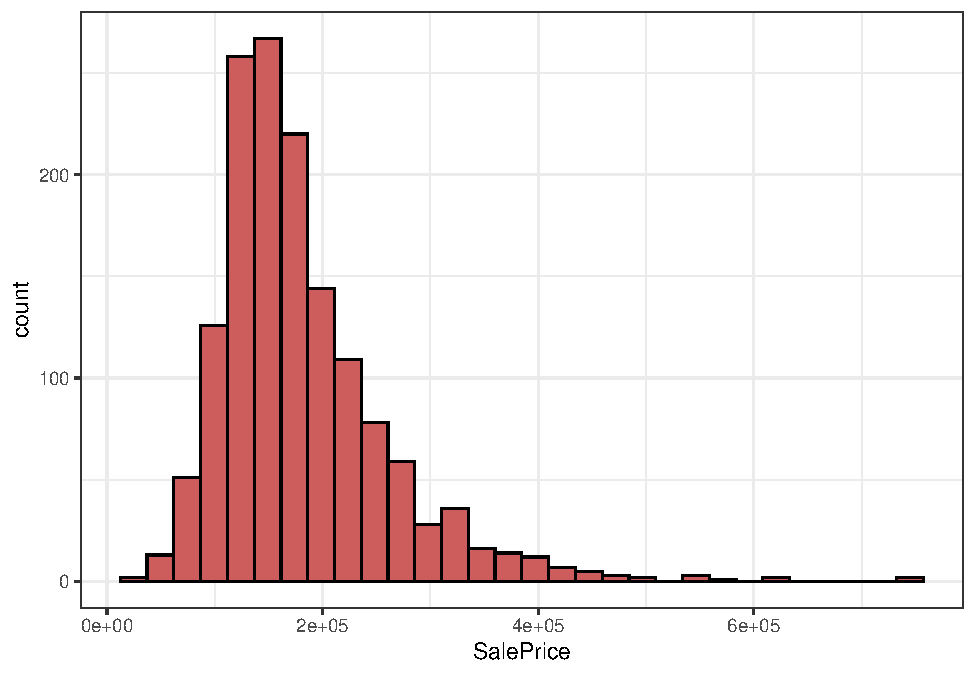
\includegraphics{report_files/figure-latex/numerical variables-1.pdf}
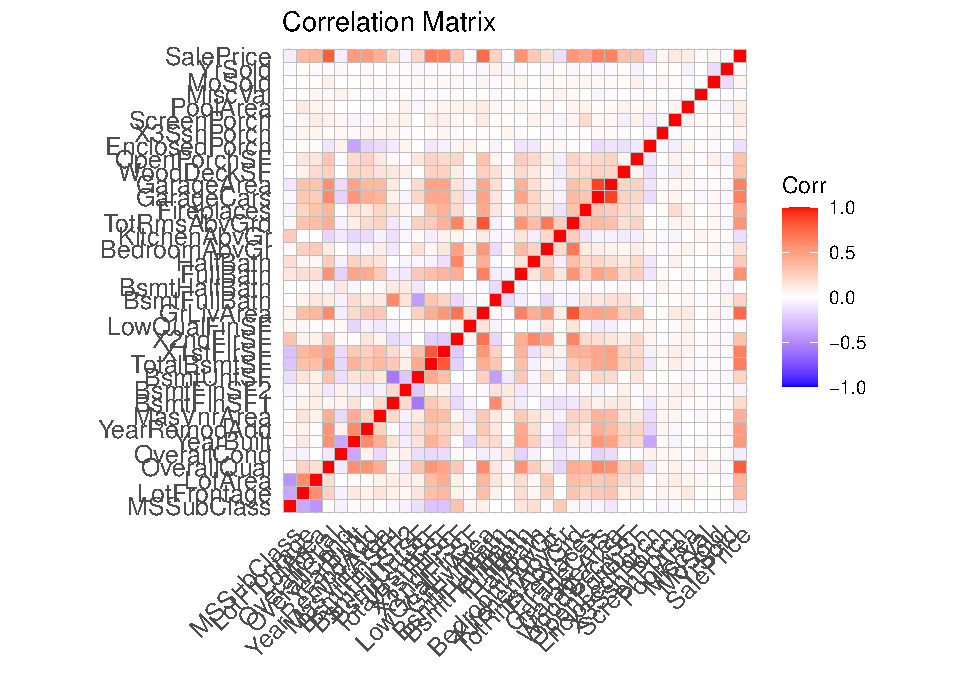
\includegraphics{report_files/figure-latex/numerical variables-2.pdf}

\begin{verbatim}
## `geom_smooth()` using formula = 'y ~ x'
\end{verbatim}

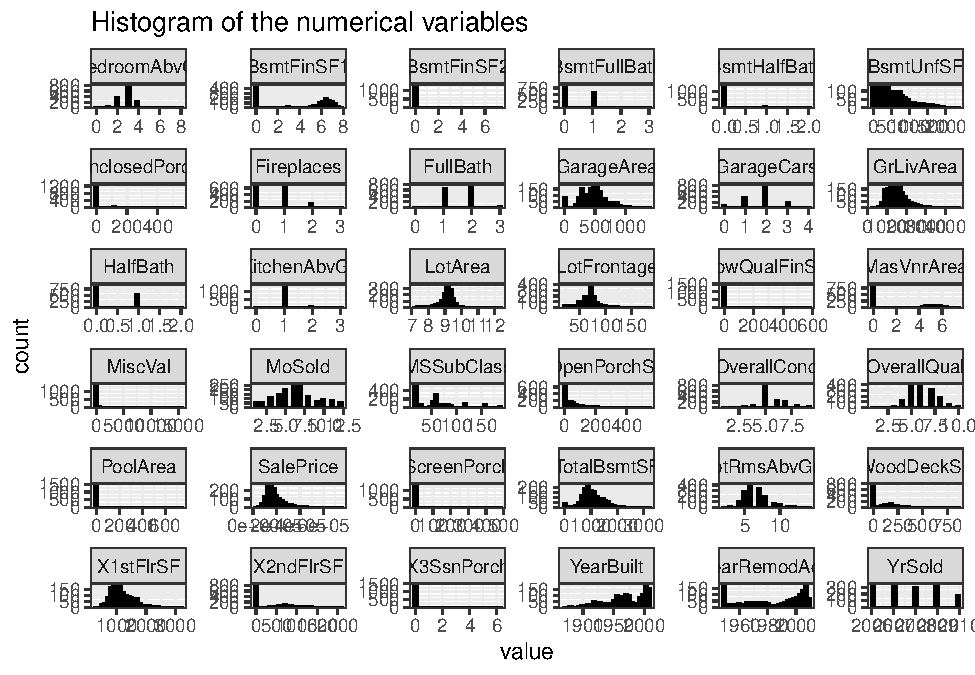
\includegraphics{report_files/figure-latex/numerical variables-3.pdf}

\begin{verbatim}
## `geom_smooth()` using formula = 'y ~ x'
\end{verbatim}

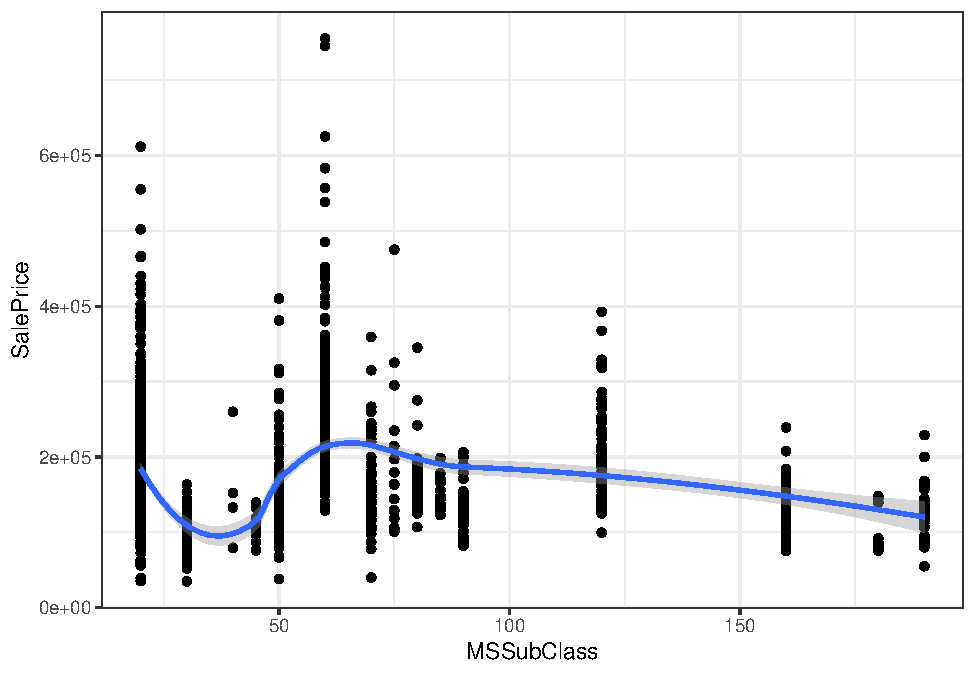
\includegraphics{report_files/figure-latex/numerical variables-4.pdf}

\begin{verbatim}
## `geom_smooth()` using formula = 'y ~ x'
\end{verbatim}

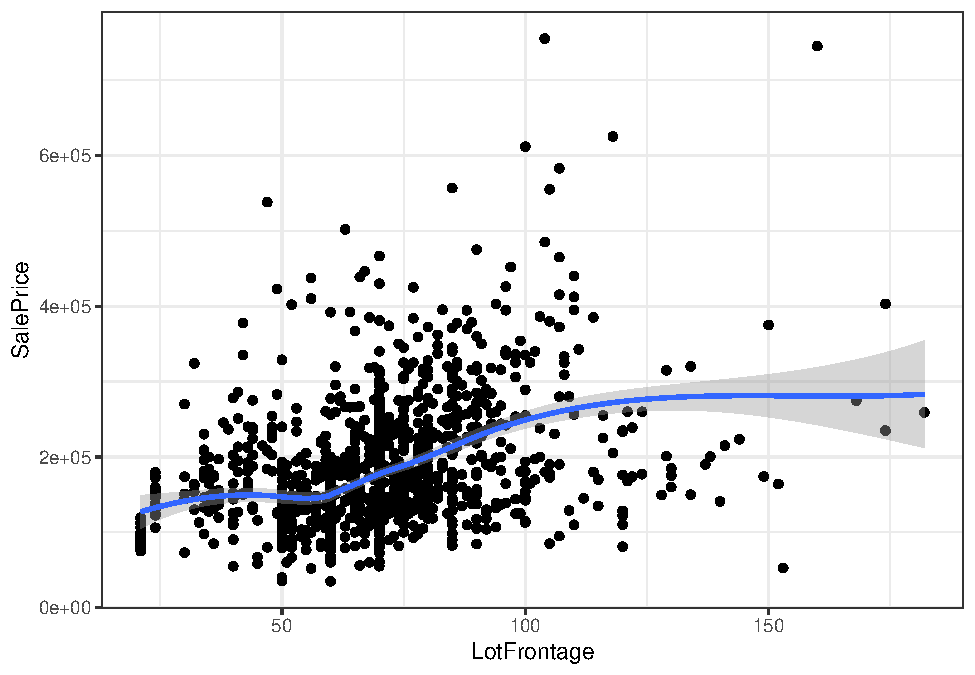
\includegraphics{report_files/figure-latex/numerical variables-5.pdf}

Since

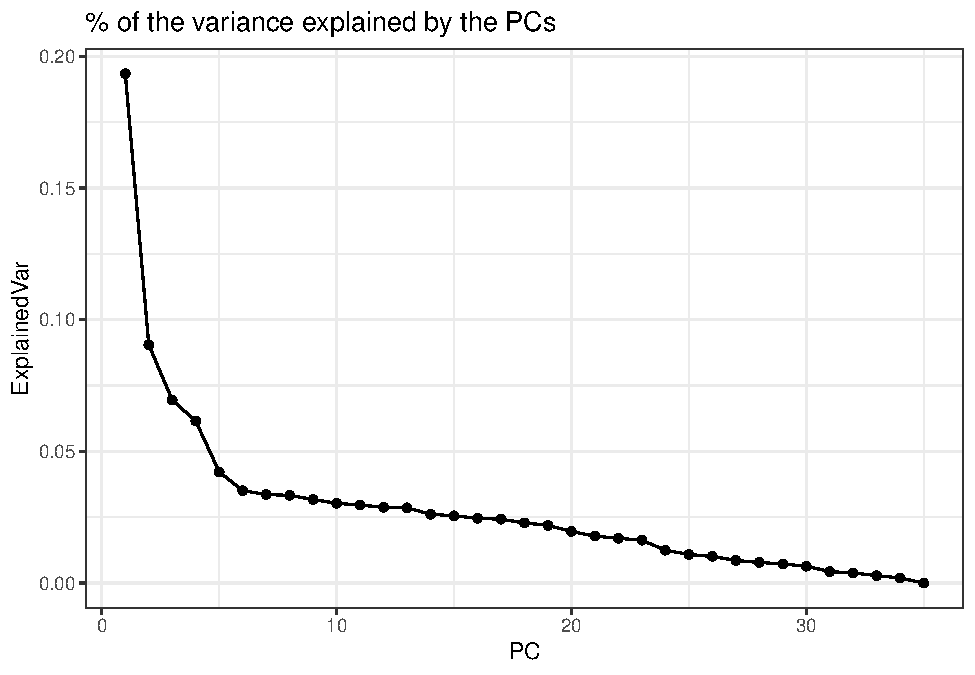
\includegraphics{report_files/figure-latex/dimensionality reduction-1.pdf}
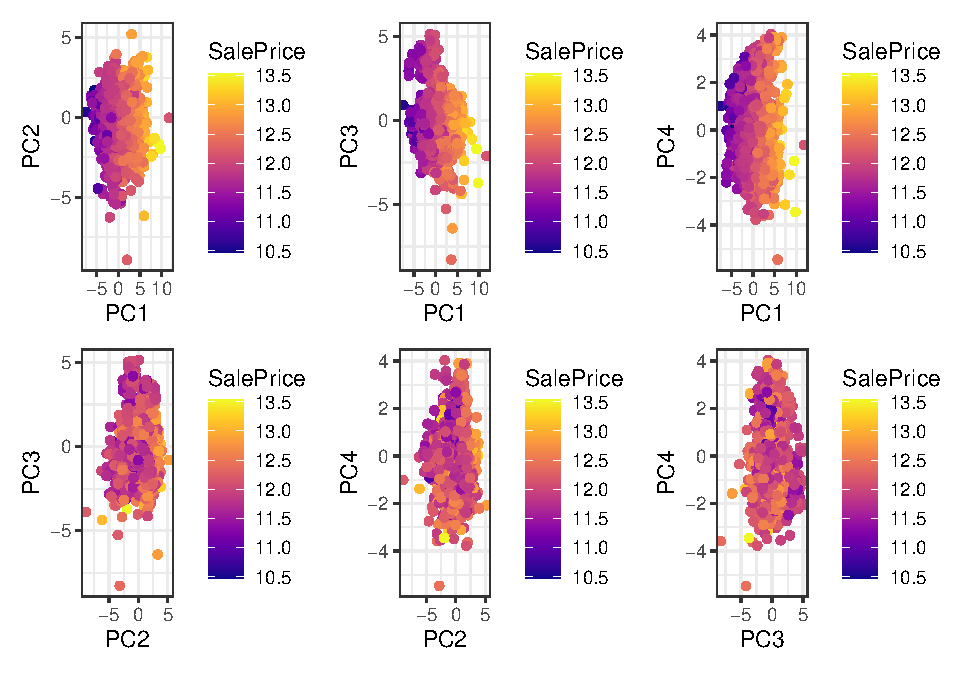
\includegraphics{report_files/figure-latex/dimensionality reduction-2.pdf}
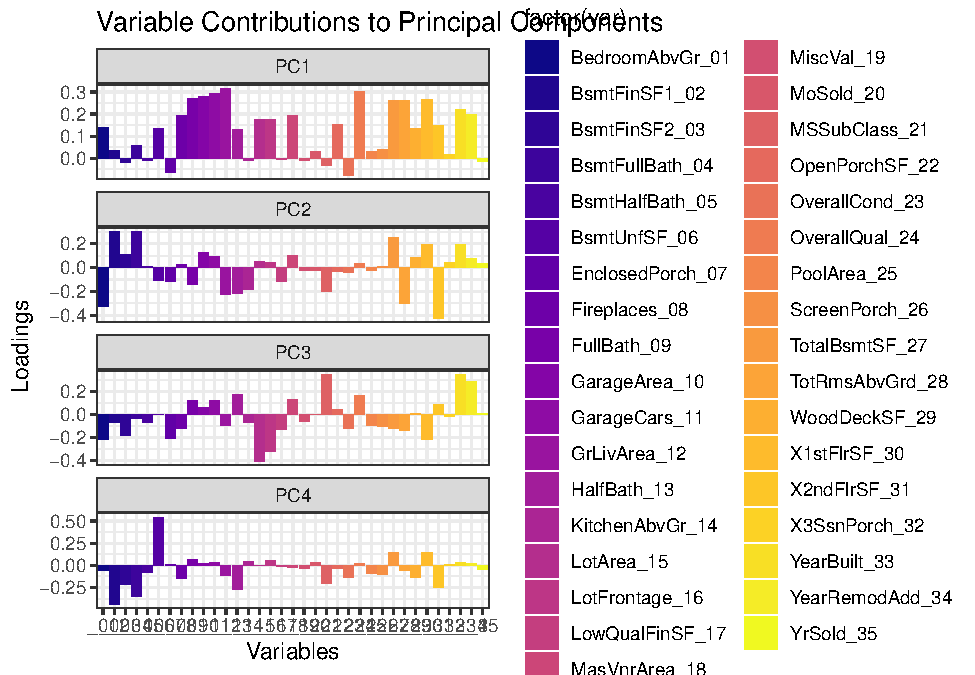
\includegraphics{report_files/figure-latex/dimensionality reduction-3.pdf}

\begin{verbatim}
## Warning: `aes_string()` was deprecated in ggplot2 3.0.0.
## i Please use tidy evaluation idioms with `aes()`.
## i See also `vignette("ggplot2-in-packages")` for more information.
## This warning is displayed once every 8 hours.
## Call `lifecycle::last_lifecycle_warnings()` to see where this warning was
## generated.
\end{verbatim}

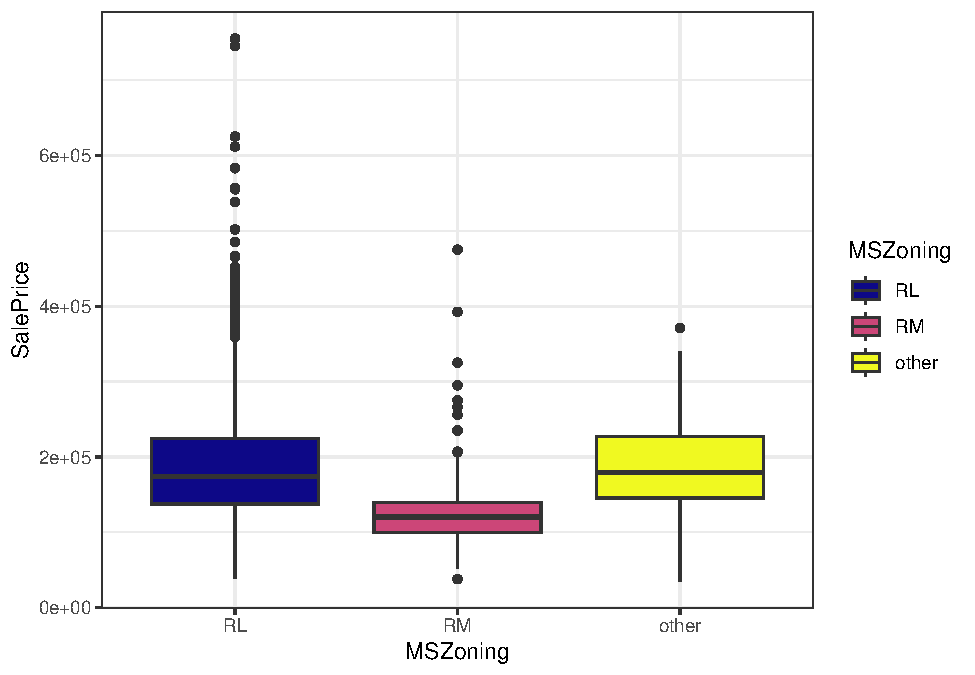
\includegraphics{report_files/figure-latex/categorical variables-1.pdf}
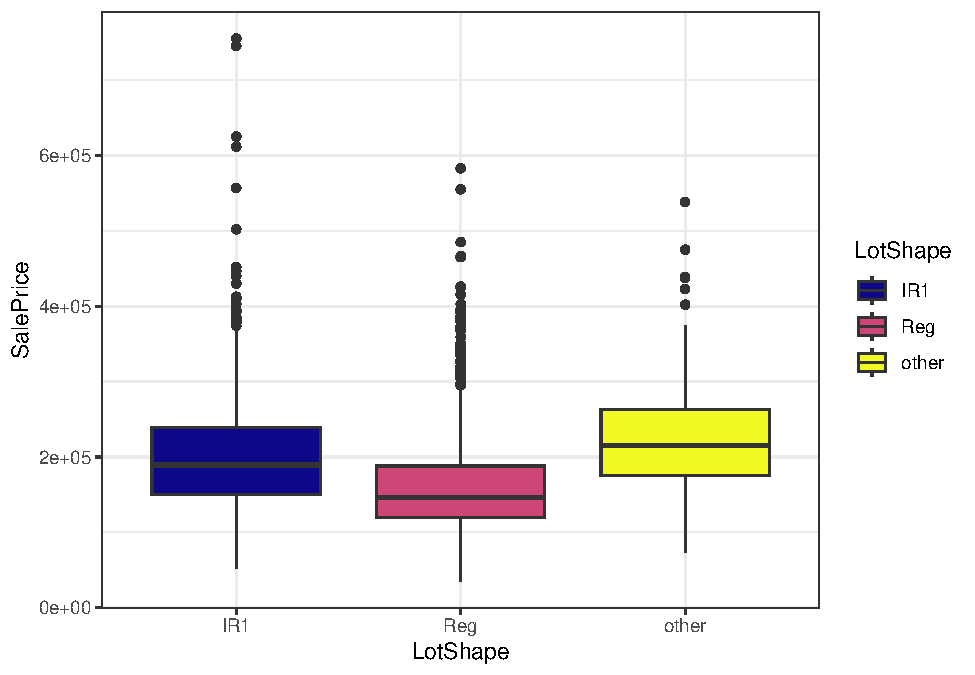
\includegraphics{report_files/figure-latex/categorical variables-2.pdf}
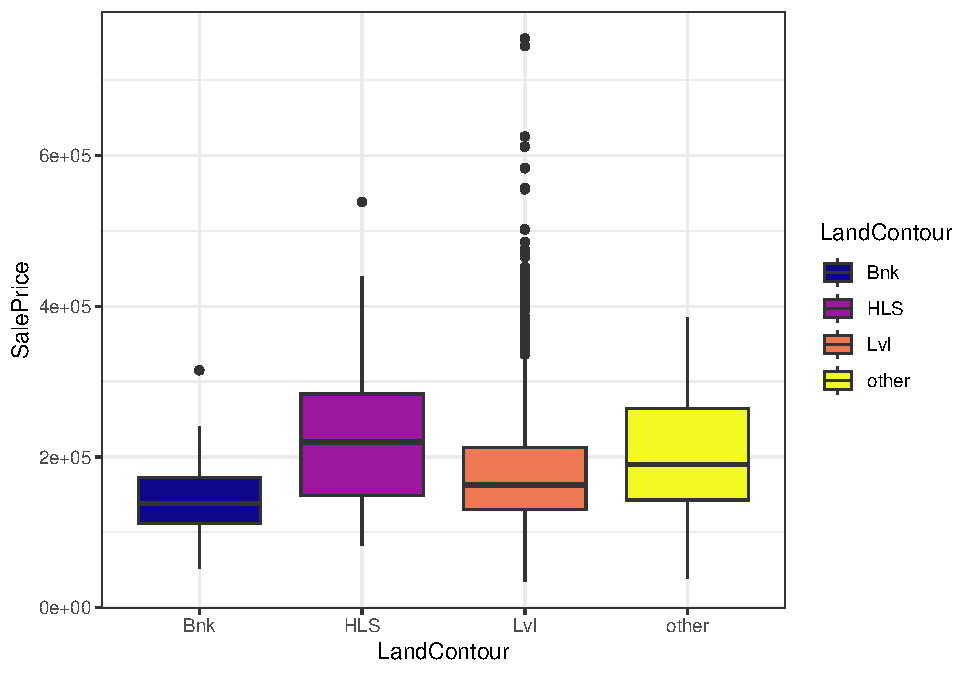
\includegraphics{report_files/figure-latex/categorical variables-3.pdf}
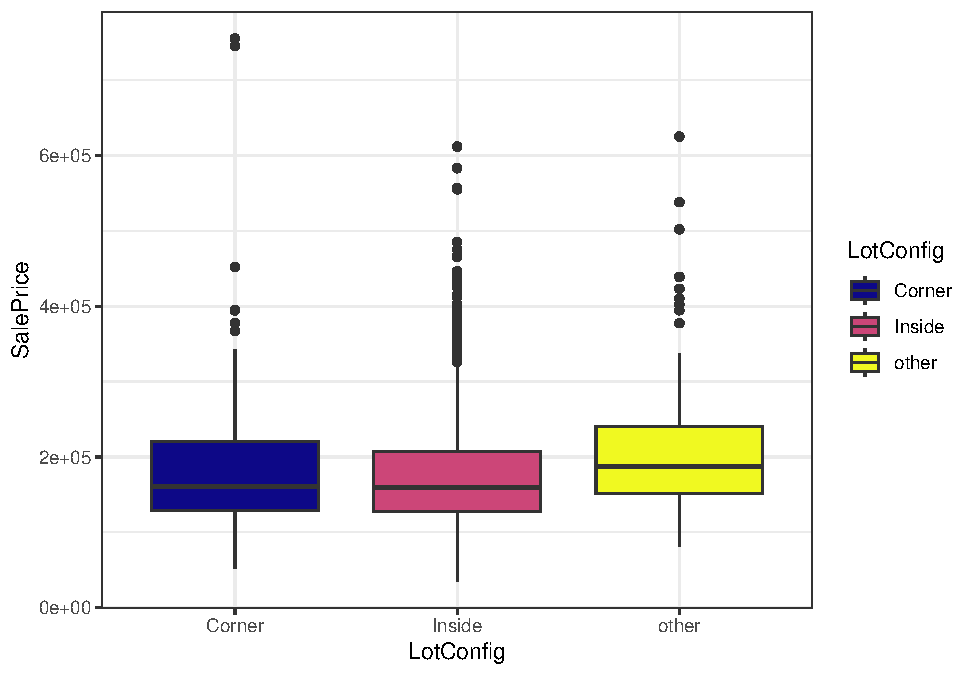
\includegraphics{report_files/figure-latex/categorical variables-4.pdf}
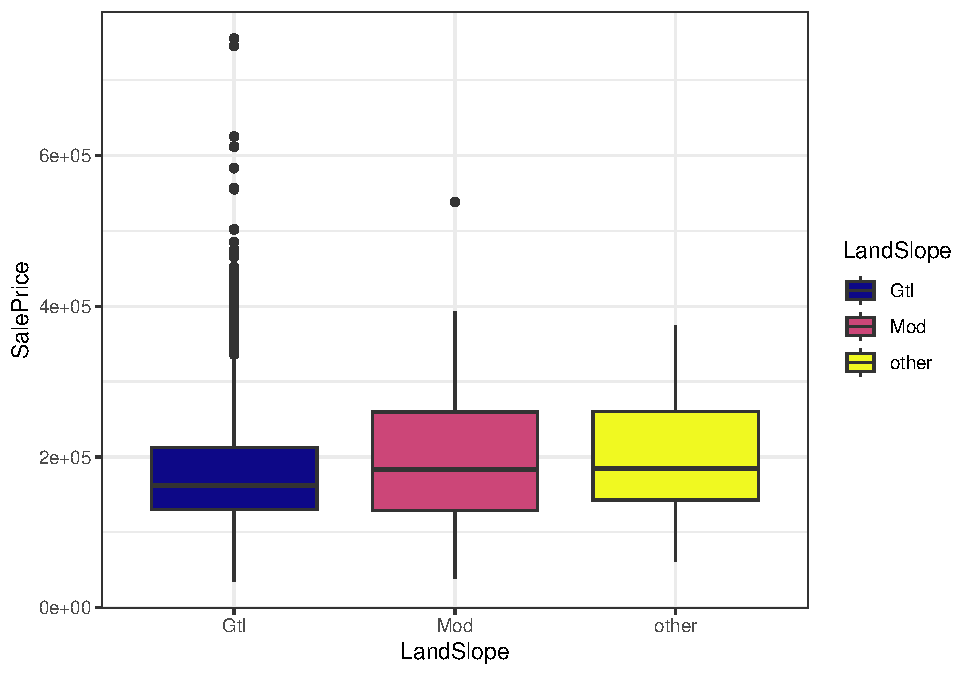
\includegraphics{report_files/figure-latex/categorical variables-5.pdf}
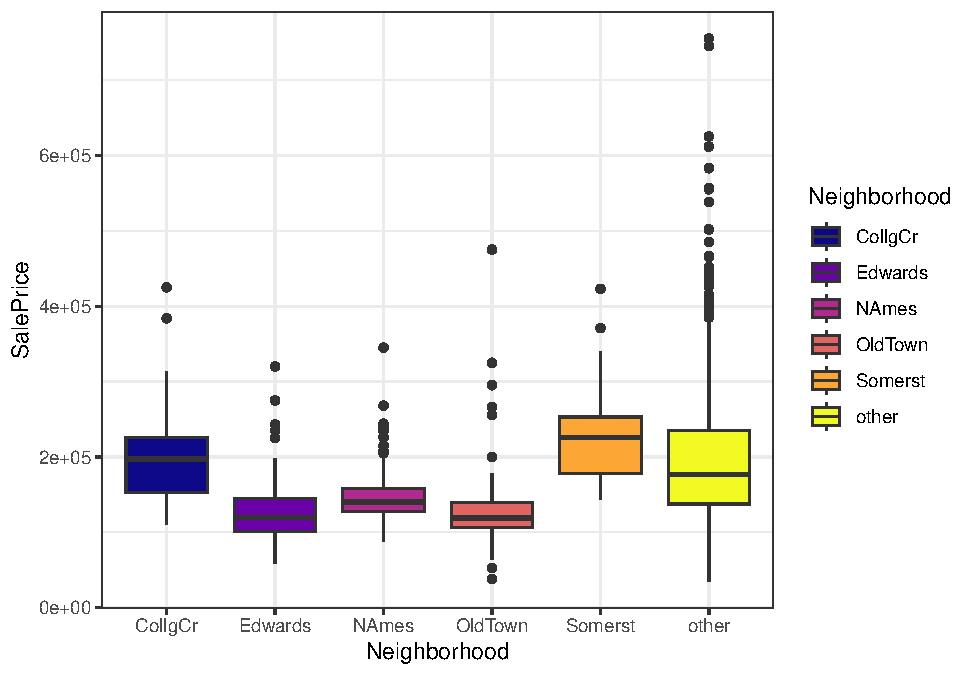
\includegraphics{report_files/figure-latex/categorical variables-6.pdf}
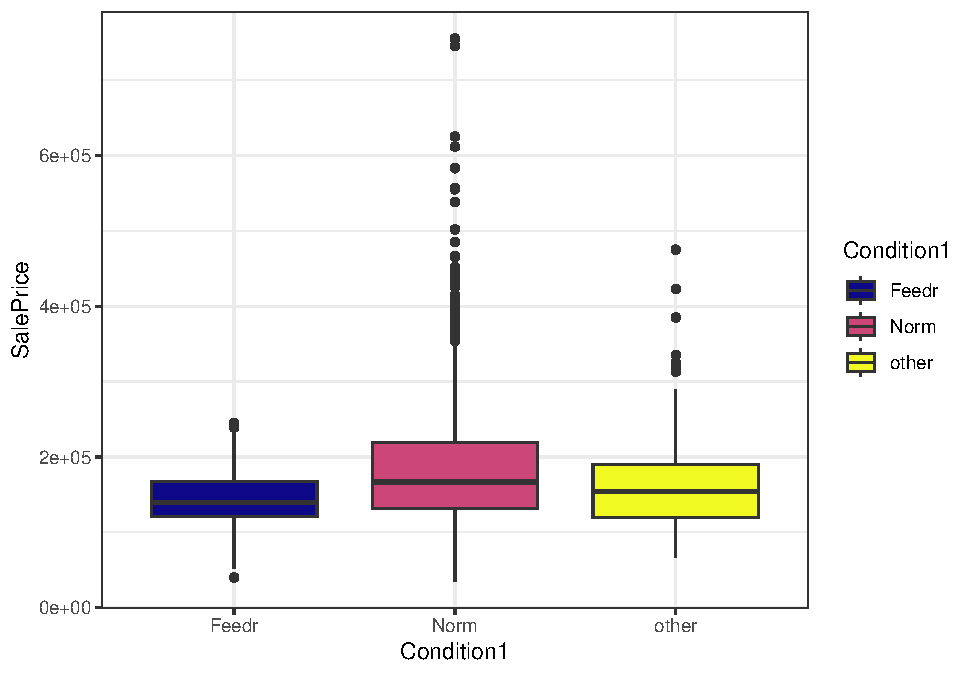
\includegraphics{report_files/figure-latex/categorical variables-7.pdf}
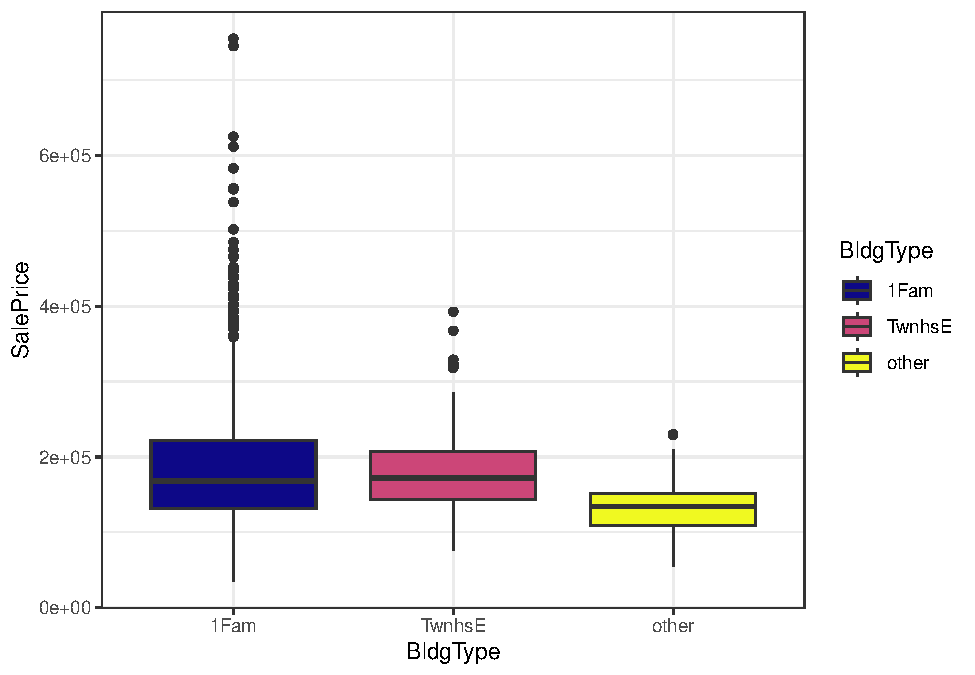
\includegraphics{report_files/figure-latex/categorical variables-8.pdf}
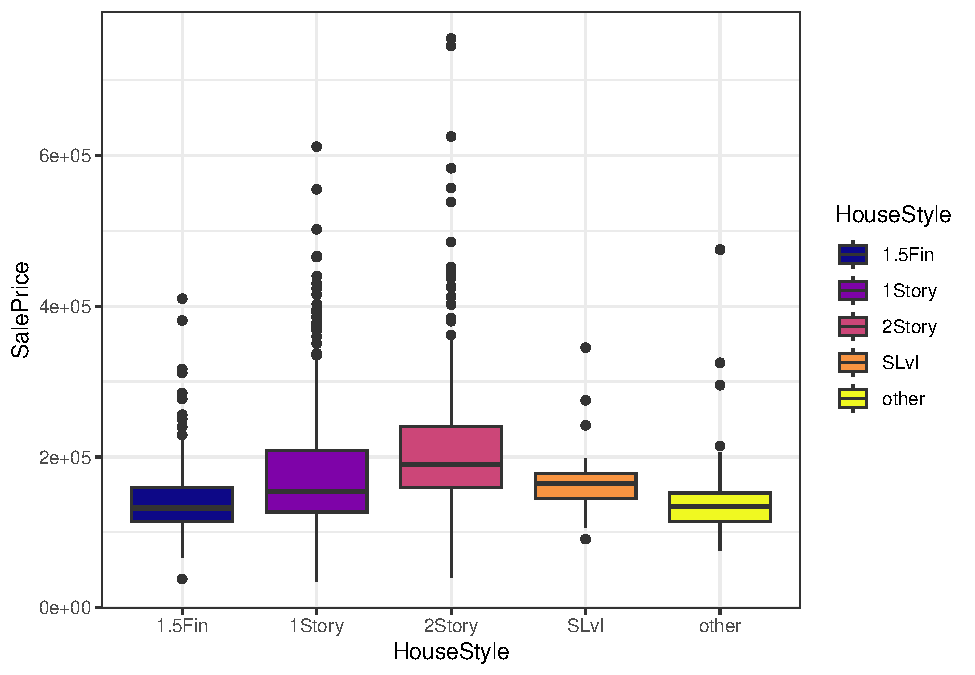
\includegraphics{report_files/figure-latex/categorical variables-9.pdf}
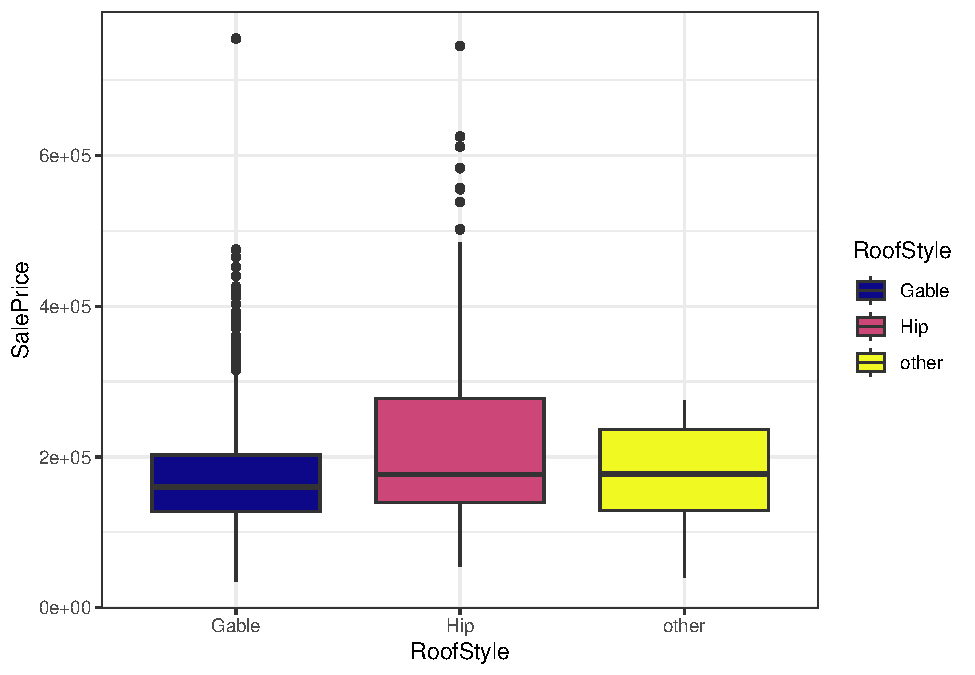
\includegraphics{report_files/figure-latex/categorical variables-10.pdf}
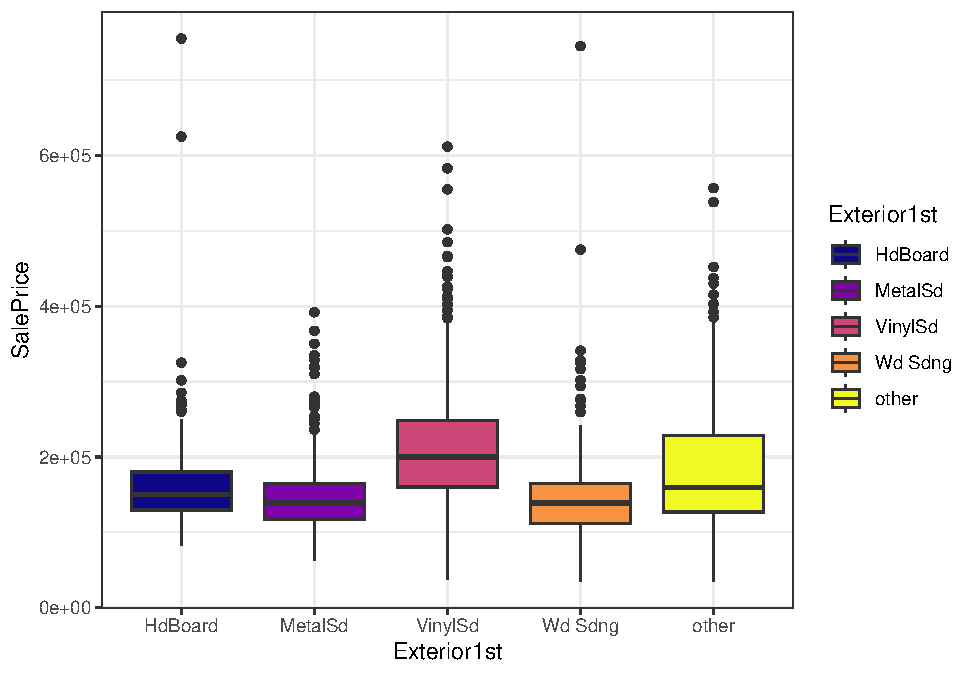
\includegraphics{report_files/figure-latex/categorical variables-11.pdf}
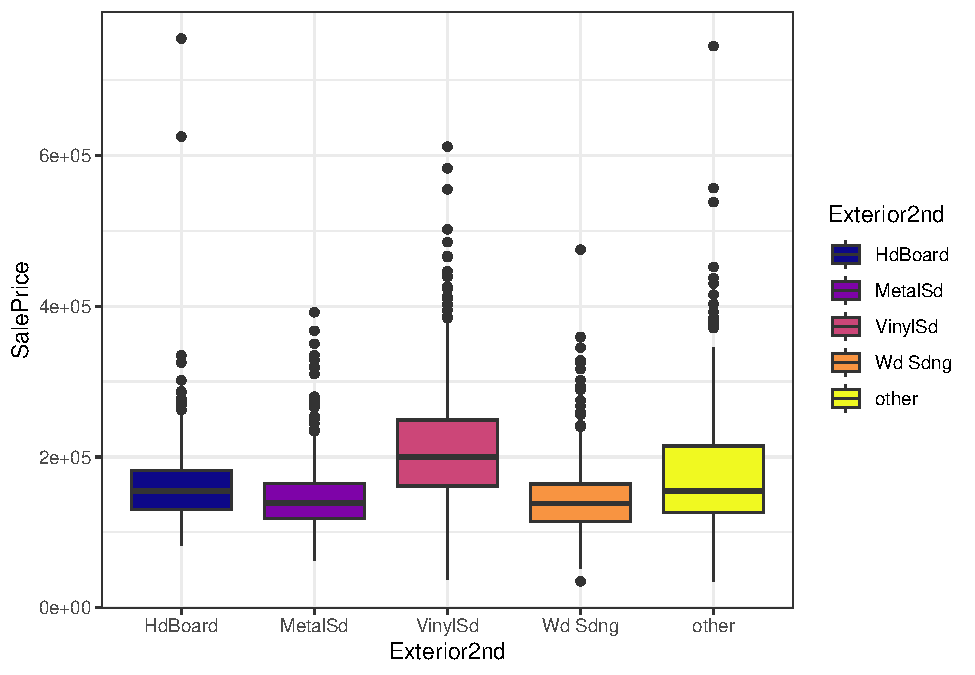
\includegraphics{report_files/figure-latex/categorical variables-12.pdf}
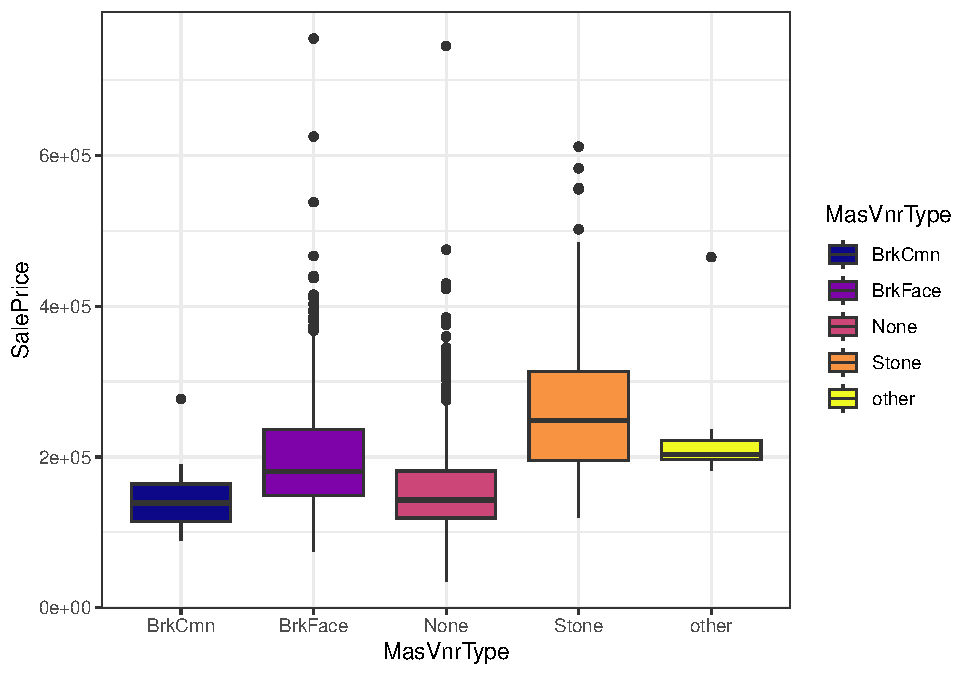
\includegraphics{report_files/figure-latex/categorical variables-13.pdf}
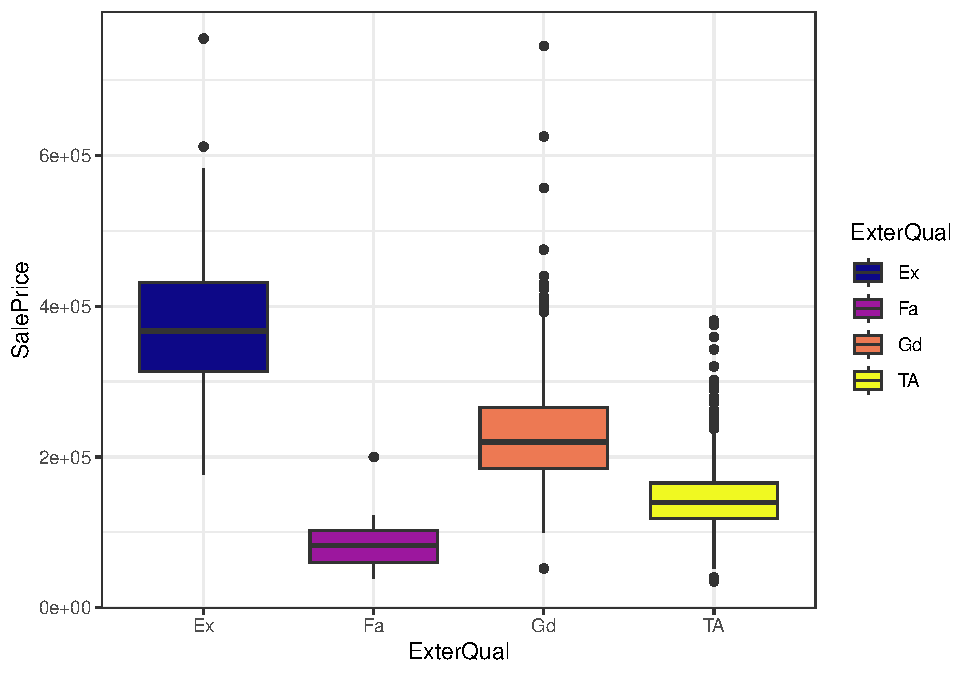
\includegraphics{report_files/figure-latex/categorical variables-14.pdf}
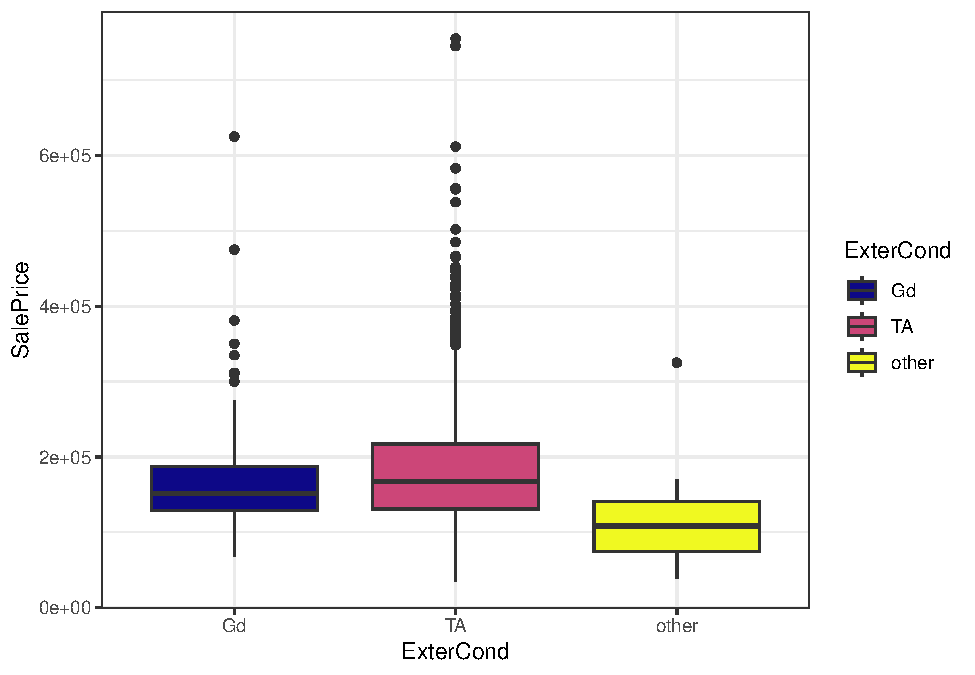
\includegraphics{report_files/figure-latex/categorical variables-15.pdf}
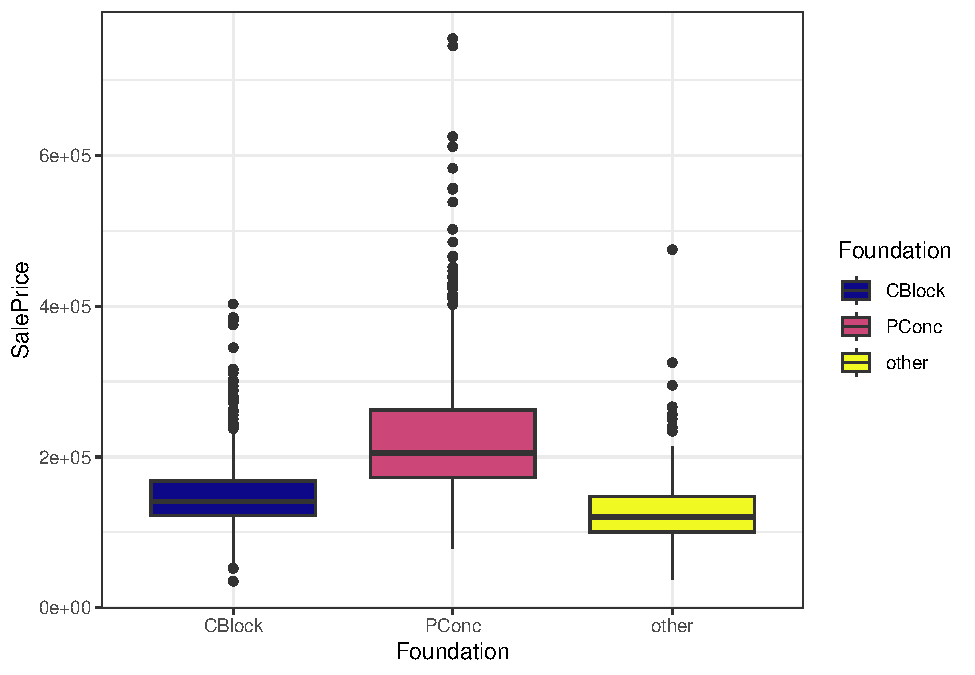
\includegraphics{report_files/figure-latex/categorical variables-16.pdf}
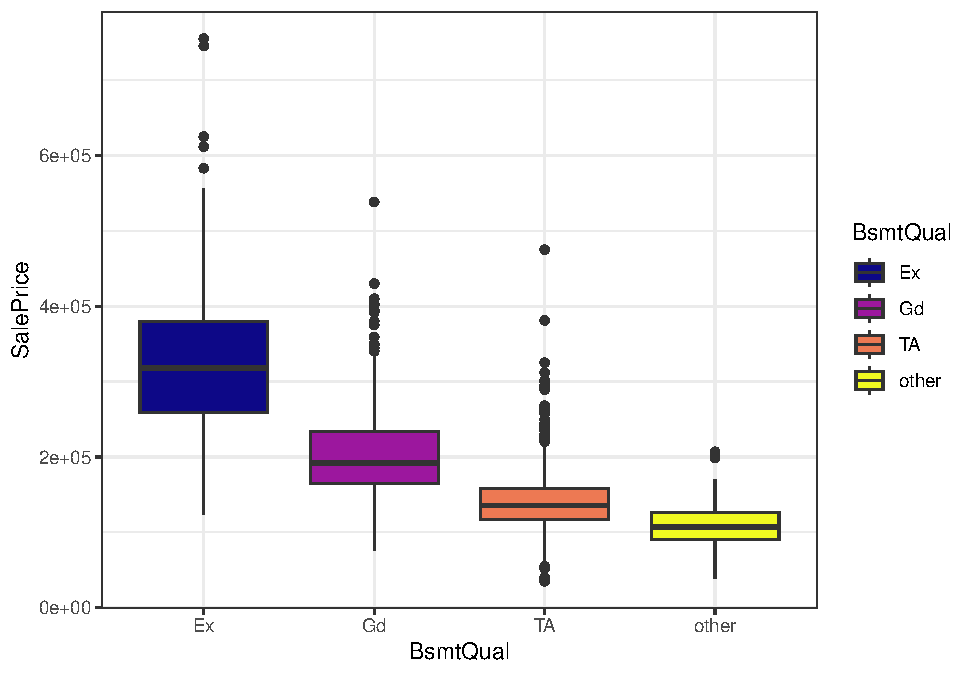
\includegraphics{report_files/figure-latex/categorical variables-17.pdf}
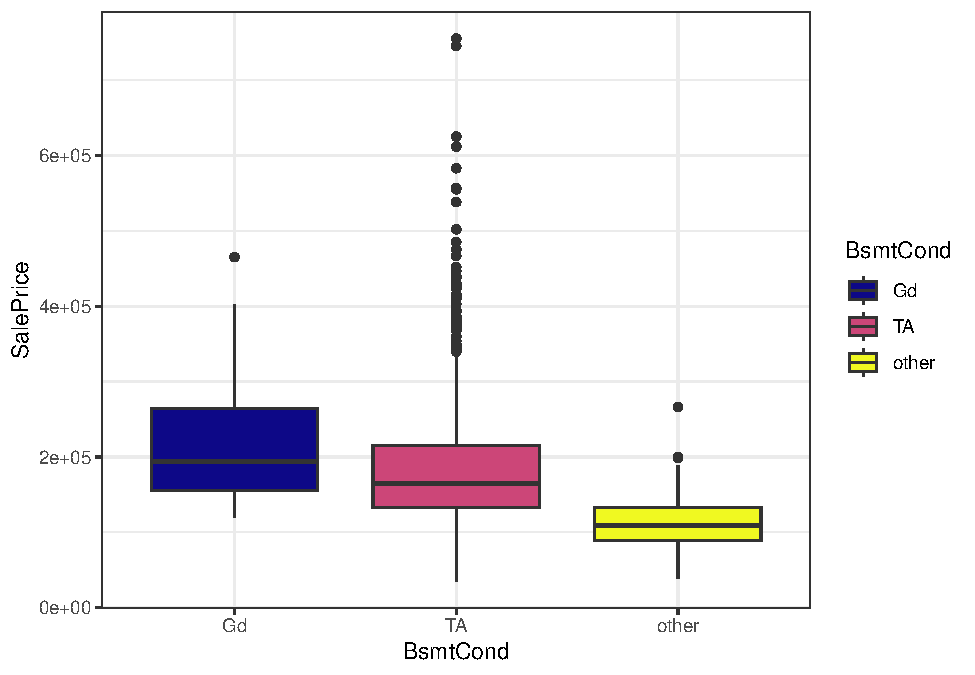
\includegraphics{report_files/figure-latex/categorical variables-18.pdf}
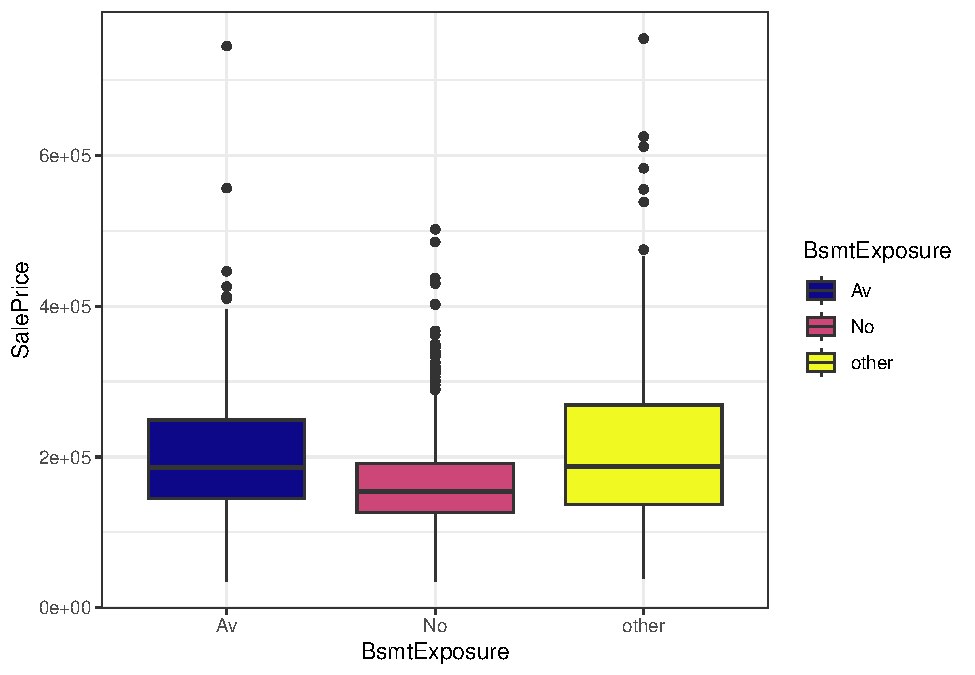
\includegraphics{report_files/figure-latex/categorical variables-19.pdf}
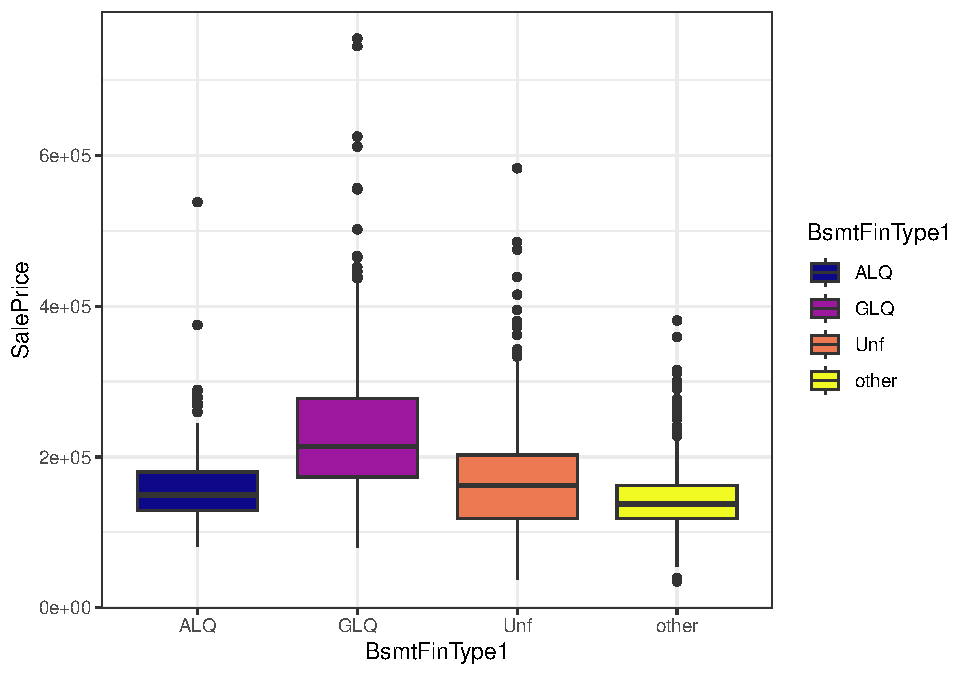
\includegraphics{report_files/figure-latex/categorical variables-20.pdf}
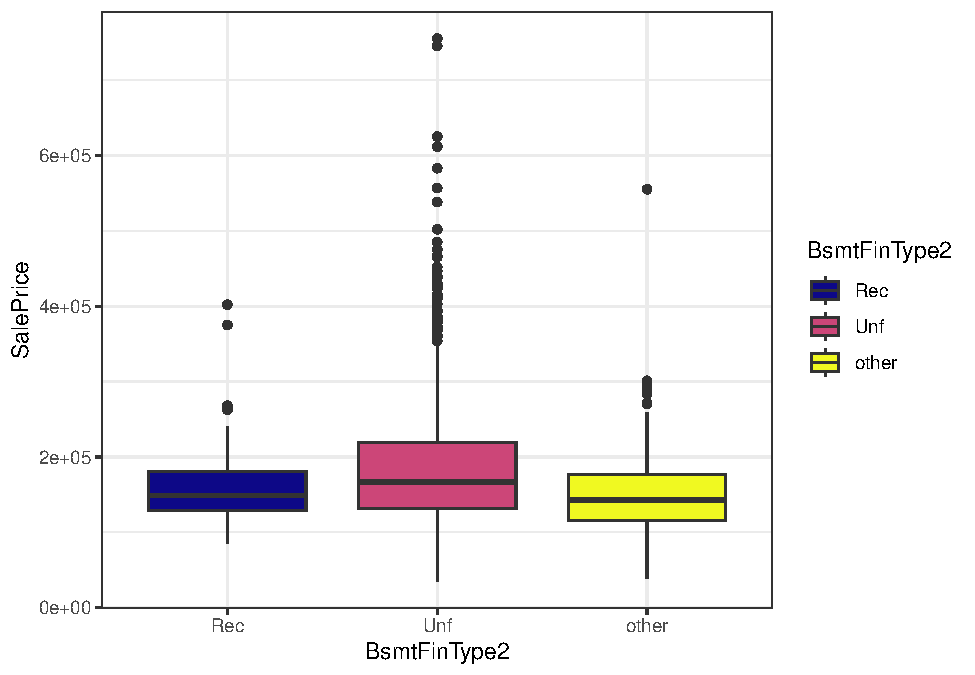
\includegraphics{report_files/figure-latex/categorical variables-21.pdf}
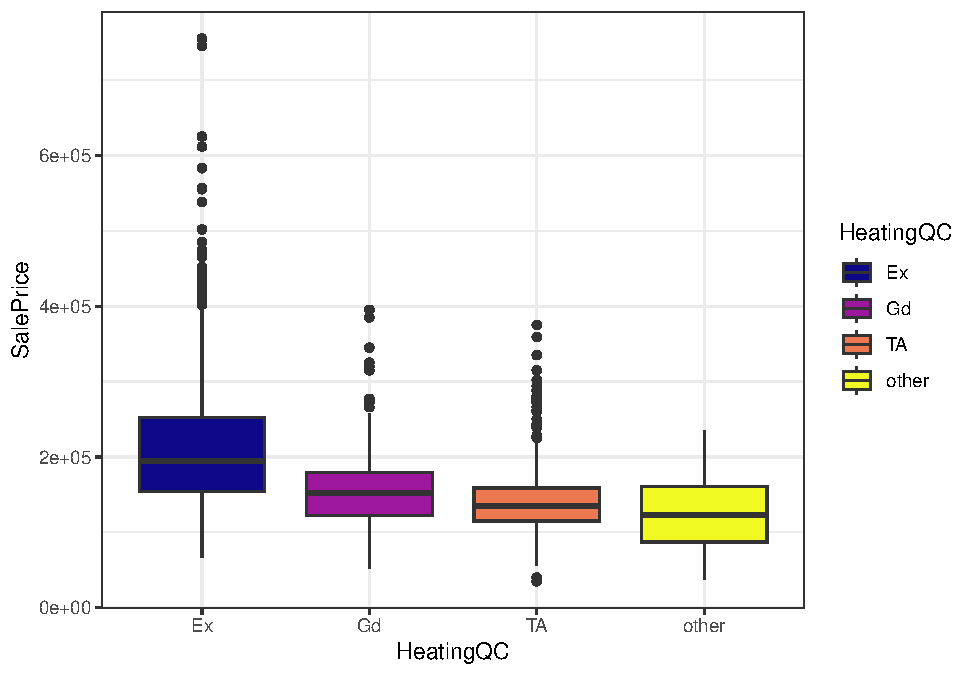
\includegraphics{report_files/figure-latex/categorical variables-22.pdf}
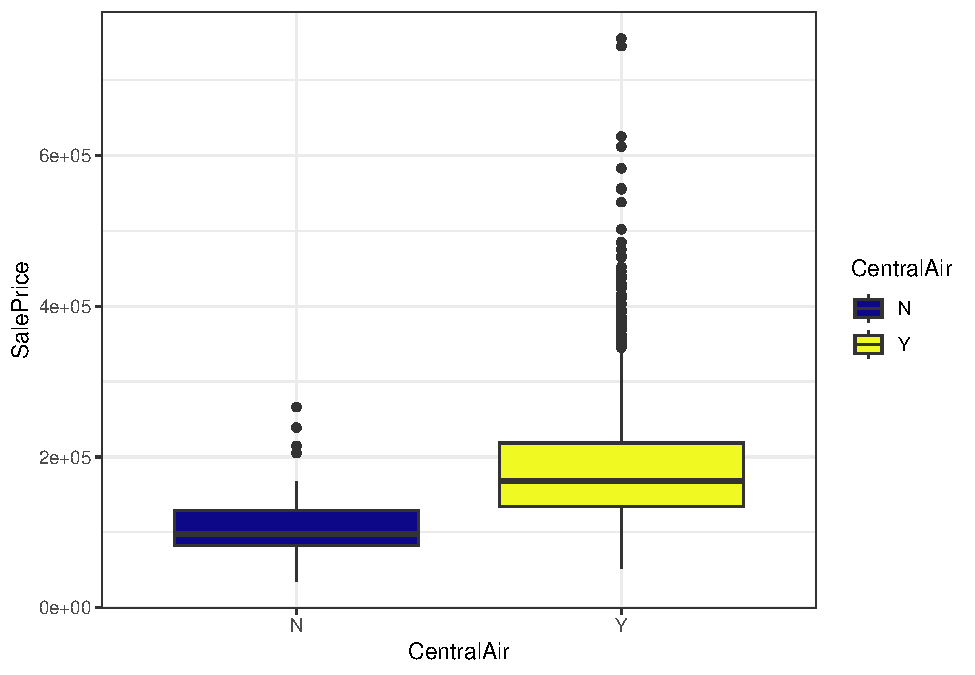
\includegraphics{report_files/figure-latex/categorical variables-23.pdf}
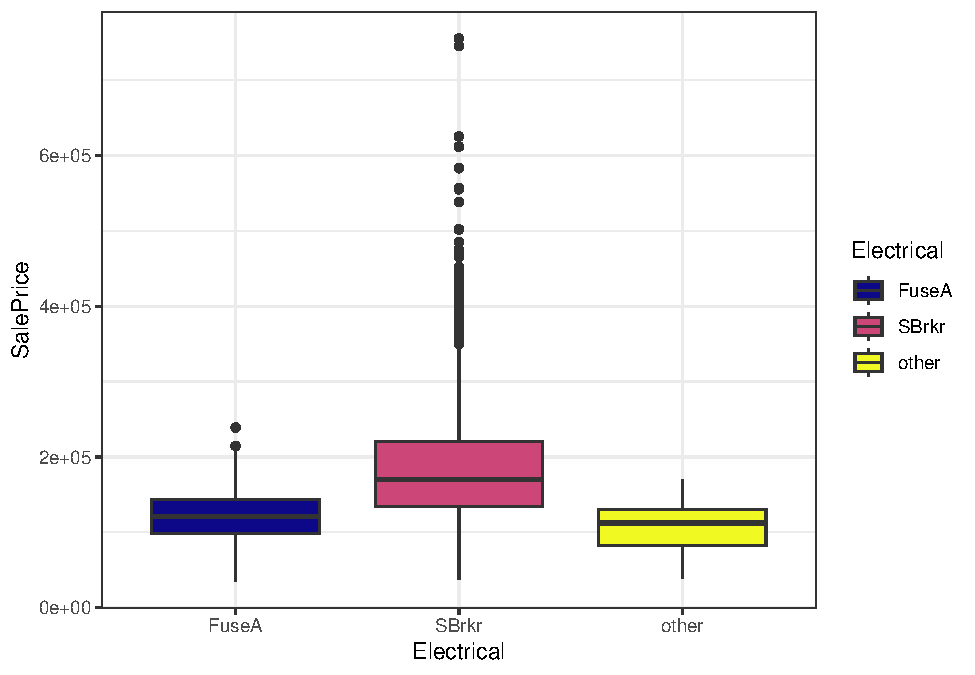
\includegraphics{report_files/figure-latex/categorical variables-24.pdf}
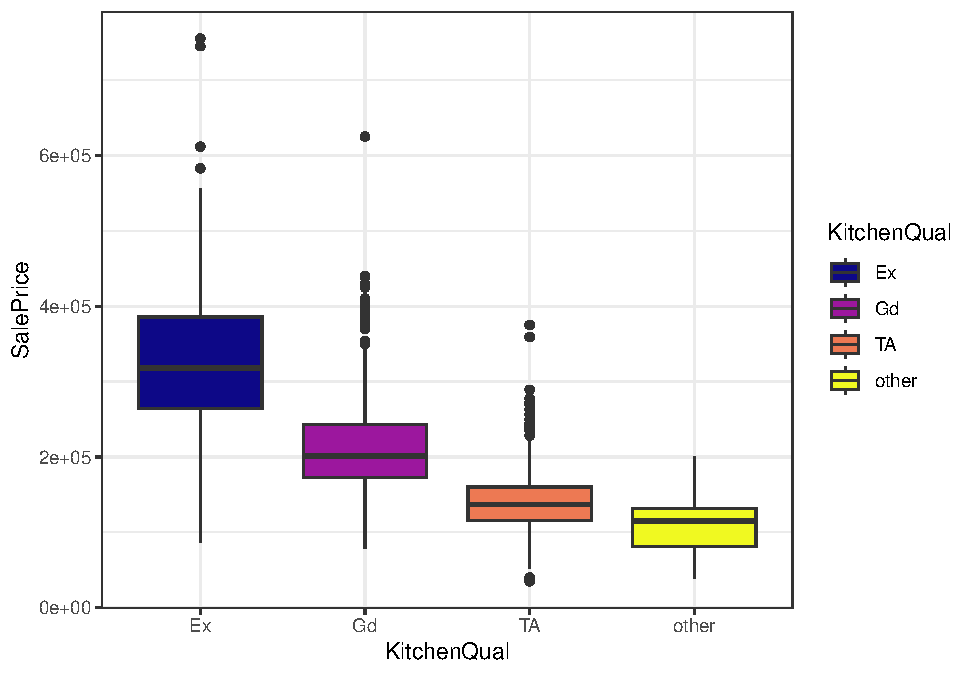
\includegraphics{report_files/figure-latex/categorical variables-25.pdf}
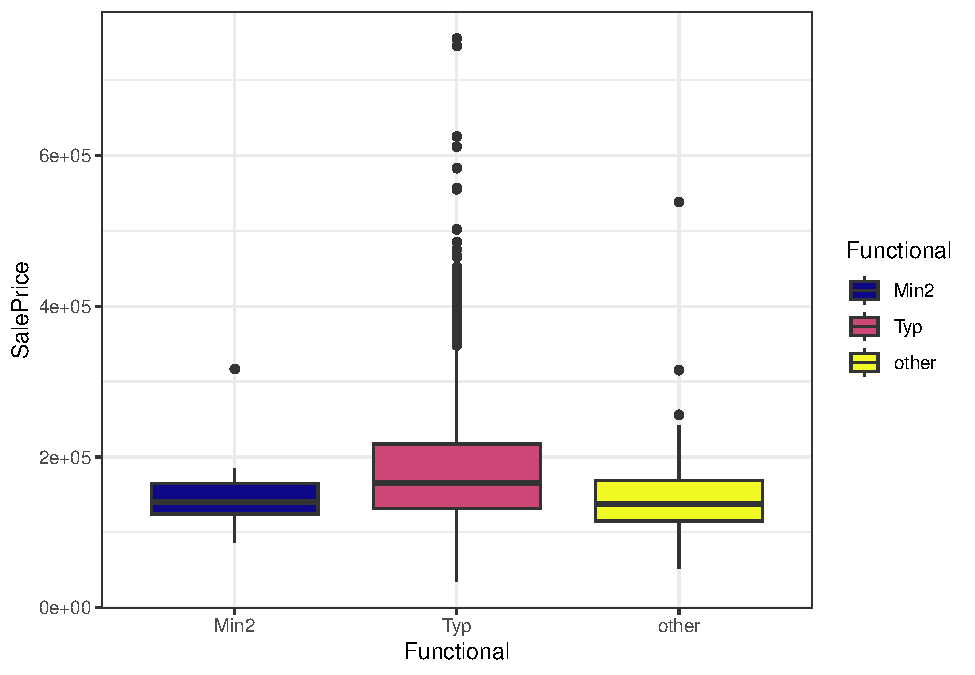
\includegraphics{report_files/figure-latex/categorical variables-26.pdf}
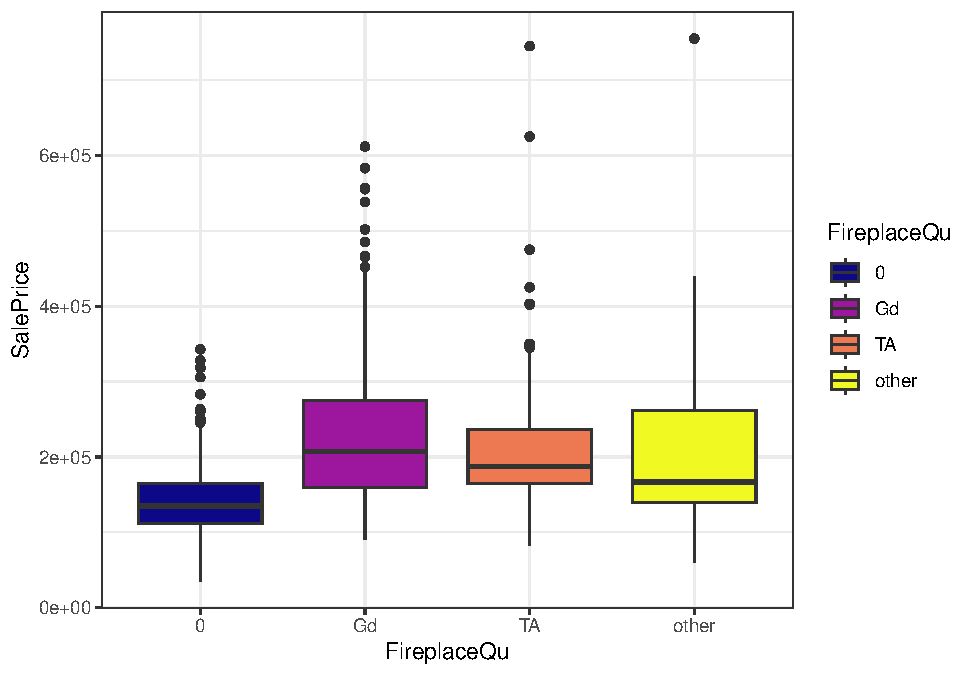
\includegraphics{report_files/figure-latex/categorical variables-27.pdf}
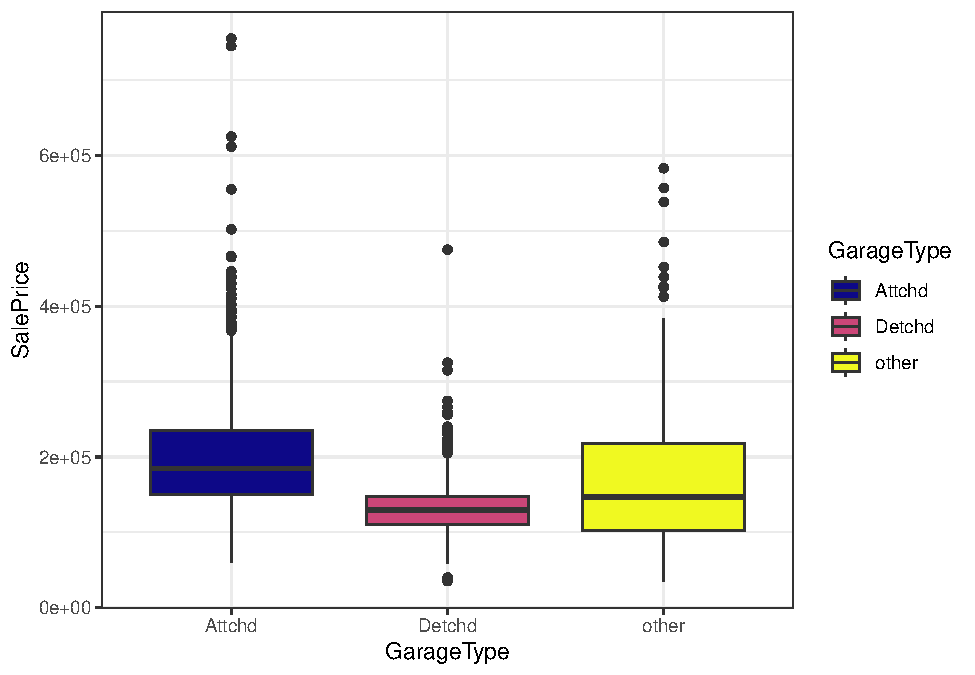
\includegraphics{report_files/figure-latex/categorical variables-28.pdf}
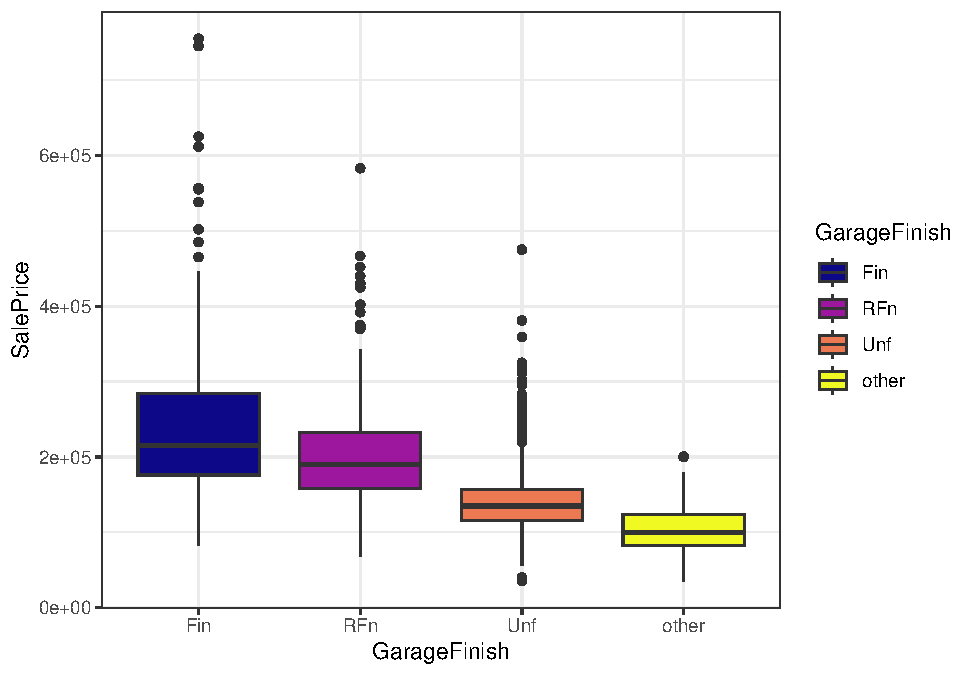
\includegraphics{report_files/figure-latex/categorical variables-29.pdf}
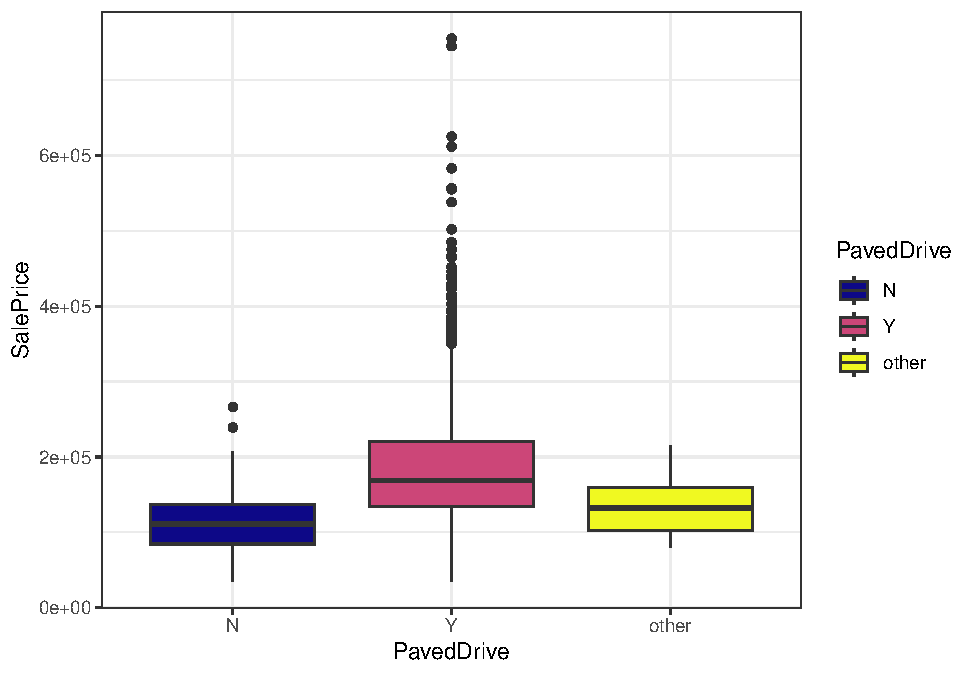
\includegraphics{report_files/figure-latex/categorical variables-30.pdf}
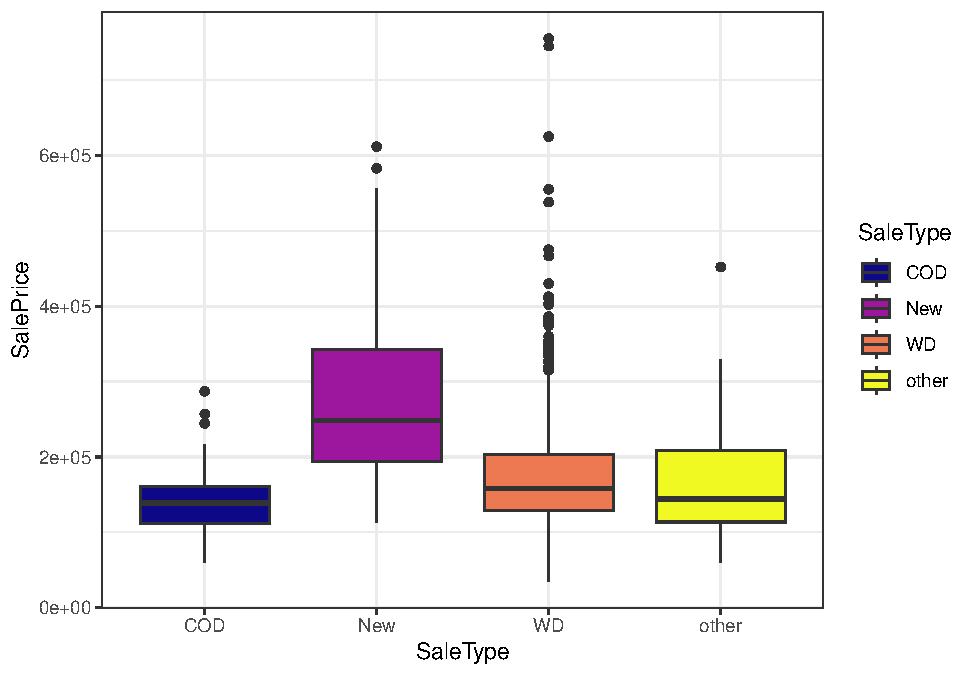
\includegraphics{report_files/figure-latex/categorical variables-31.pdf}
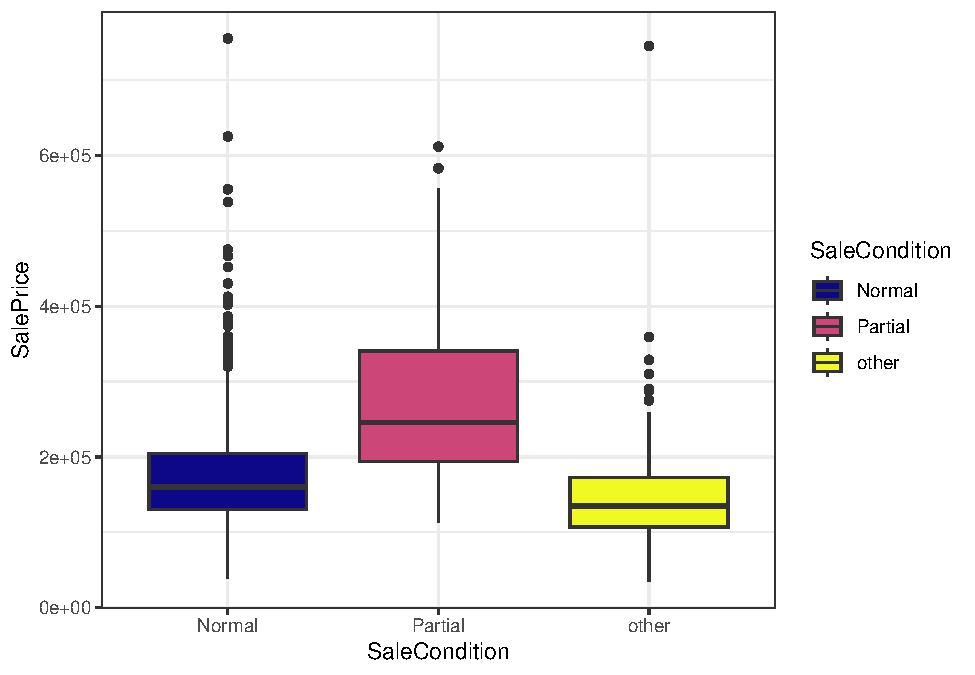
\includegraphics{report_files/figure-latex/categorical variables-32.pdf}
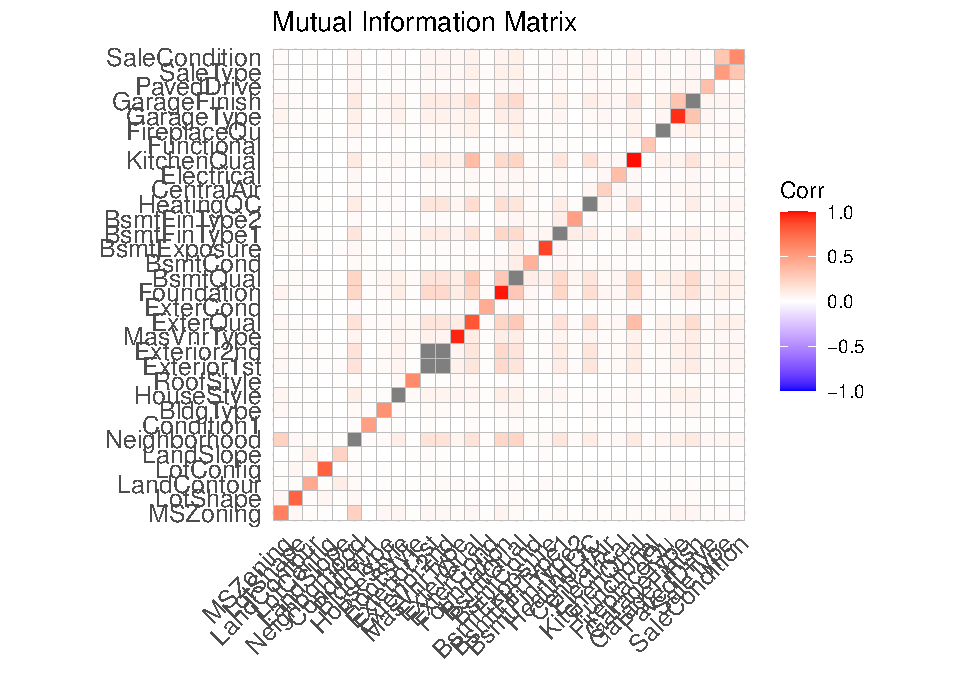
\includegraphics{report_files/figure-latex/categorical variables-33.pdf}

\begin{Shaded}
\begin{Highlighting}[]
\NormalTok{knitr}\SpecialCharTok{::}\FunctionTok{knit\_exit}\NormalTok{()}
\end{Highlighting}
\end{Shaded}

\phantomsection\label{refs}
\begin{CSLReferences}{0}{1}
\bibitem[\citeproctext]{ref-kaggledata}
1. Anna Montoya D.
\href{https://kaggle.com/competitions/house-prices-advanced-regression-techniques}{House
prices - advanced regression techniques}. 2016.

\end{CSLReferences}

\end{document}
